\documentclass[12pt,fleqn]{article}
\usepackage[utf8]{inputenc}
\usepackage[frenchb]{babel}
\usepackage[T1]{fontenc}
\usepackage{array}
\usepackage{color}
\usepackage{calc}
\usepackage{color,linegoal}
\usepackage{titling}
\usepackage{url}
\usepackage{float}
\usepackage{graphicx}
\usepackage{setspace}
\setlength{\droptitle}{-2.8cm}
\setlength{\textwidth}{6.5in}
\setlength{\textheight}{9in}
\renewcommand{\baselinestretch}{1.5}
\setlength{\unitlength}{1mm}
\setlength{\topmargin}{-14mm}%24
\setlength{\oddsidemargin}{-0.0001in}% 1mm
\setlength{\parskip}{1mm}
\newcommand{\GG}{\guillemotleft\xspace}
\newcommand{\GD}{\guillemotright\xspace}
\newcommand{\CT}[1]{\GG~{#1}~\GD\xspace}



\definecolor{lightgray}{gray}{0.90}
\definecolor{SolutionColor}{gray}{0.85}
\renewcommand{\baselinestretch}{1.5}

\begin{document}
\def\always{{\vcenter{\vbox{\hrule height.4pt
                   \hbox{\vrule width.4pt height9pt \kern9pt
                         \vrule width.4pt}
                         \hrule height.4pt}}}}

\def\undertext#1{$\underline{\hbox{#1}}$}



\begin{center}

\includegraphics[height=2.5cm,width=2.5cm]{images/Athlimage-logo.png}
\end{center}


\begin{center}
{\bf\LARGE    Athlimage }
\vspace{1cm}

par
\vspace{1cm}

Dordor Minetdi 

Alexandre Beauquel

Alexandre Roussel 

Sébastien O'Neel

\vspace{1cm}
{\large Travail présenté à

Gabriel Girard

\vspace{0.5cm}

 dans le cadre de l'activité pédagogique
 \vspace{0.3cm}


{\bf IFT592 - Projet d'informatique I}


\vspace{1cm}


D\'EPARTEMENT D'INFORMATIQUE

UNIVERSIT\'E DE SHERBROOKE

\vspace{0.5cm}


\today}

\end{center}

\newpage

\renewcommand{\baselinestretch}{1.2}
\normalsize


\tableofcontents

\newpage

\section{Introduction}

Athlimage est une entreprise de photographie sportive. Une grande partie de ses activités consiste à en prendre des photos lors d’événements sportifs et de les vendre sur place (la production et l’impression des photos sont également sur place). Pour ce faire, l’entreprise se déplace à de nombreux événements et divers emplacement. Que ce soit des arénas pour des tournois de hockey, des terrains extérieurs pour des compétitions d’athlétisme, des écoles pour des tournois de basketball et divers autres types d’endroit. L’entreprise a besoin d’un système mobile. Présentement, les commandes sont écrites sur un papier qui est passé au graphiste qui s’occupe de produire les photos. Lorsque le nombre de commandes est faible, il est plutôt facile à gérer, mais lorsqu’il y a un grand nombre de commandes les problèmes commencent à apparaitre. Mélange dans l’ordre des commandes, perte d’une commande ou oublie d’une commande (présumé faite alors qu’elle ne l’est pas). Tous ces problèmes arrivent relativement fréquemment lors des événements et causent des frustrations chez les clients. Pour régler ce problème, il a été décidé de créer une application mobile et de bureau, communiquant ensemble et permettant à un employé de prendre les commandes et les envoyer directement au graphiste, réglant ainsi les problèmes mentionnés ci-haut.


Or un problème apparait. Puisque l’entreprise se déplace à une grande variété d’endroits, il est impossible de garantir l’accès à un réseau Wi-Fi en tout temps. Dans certaine école le Wi-Fi est verrouillé, dans certaine aréna le Wi-Fi est très variable et sur un terrain d’athlétisme, il n’y a généralement pas de Wi-Fi. Il faut donc trouver un moyen que les deux applications communiquent ensemble sans passer par Internet. Il y a donc été choisi que les applications communiqueront via Bluetooth. L’entreprise se sert d’appareil Apple, les applications devront donc être sur iOS et macOS.


Le livrable est donc deux applications, une sur mobile iOS et une sur ordinateur macOS. L’application mobile doit être capable de prendre des commandes (numéro de photo, format, forfait, etc.) et de les envoyer à l’ordinateur. L’application d’ordinateur doit pouvoir recevoir des commandes et les afficher. On doit pouvoir consulter les commandes et changer leur statut une fois traité. La communication doit être faite via Bluetooth.
\newpage


\section{Revue de la littérature}

%Cette section fait une revue des documents que vous avez consulté qui traitent du même sujet ou qui ont servi de base à votre sujet.  Tous ces documents doivent être cités dans le texte et se retrouver dans la bibliographie.

%Si pertinent, elle fait aussi une revue des systèmes similaires à celui que vous avez conçu.  Vous devez justifier l'utilisation ou la non-utilisation de ces systèmes pour concevoir le vôtre.

%Ainsi, plusieurs documents ont servi pour mes travaux.
\subsection{Application mobile}
Il existe plusieurs frameworks pour le développement mobile. Puisque l’objectif de notre projet est d’avoir une application qui puisse rouler à la fois sur Android et sur iOS, il est important de choisir un framework qui facilite le plus possible le crossplateforme. Lors de mes recherches, il y a plusieurs frameworks recommandés qui reviennent toujours. Deux d’entre eux ont été examinés, Xamarin et React Native.
Pour commencer, il y a Xamarin. Ce framework utilise le langage C\# et .NET et comporte plusieurs avantages. 
\begin{enumerate}
	\item Il est fait pour le crossplateforme. L’une des fonctionnalités principales de ce framework est d’être pensée pour le crossplateforme. La grande majorité du code est partagé, peu importe la version avec seulement quelques fonctions uniques à chaque version (Android et iOS).
 	\item Il peut facilement utiliser un grand nombre de librairies (C++, Java)
	\item Il est beaucoup utilisé et par conséquent, il y a beaucoup d’aide en ligne disponible (forum, etc.)
\end{enumerate}
Ensuite, il y a React Native qui utilise le langage JavaScript. Voici quelques avantages :
\begin{enumerate}
	\item Il focus sur l’UI qui permet de concevoir des UI plus complètes.
	\item Il a un très bon crossplateforme qui ne requiert pas de coder une seule fois le code pour les 2 versions
	\item Il a également une grande communauté.
\end{enumerate}



\subsection{BluetoothLE}
En 2001, des chercheurs à Nokia ont déterminé plusieurs scénarios que le sans-fil moderne n'adressait pas. La compagnie a donc commencé à développer une technologie sans-fils adaptées du standard de Bluetooth en utilisant moins d'énergie et a un cout plus faible en minimisant la différence entre les deux. Les résultats ont été publiés en 2004 avec le nom Bluetooth Low End Extension\cite{BLEStart}. Après plus de développement avec Logitech en collaboration avec le projet MIMOSA tout en étant supporté et promu par STMicroelectronics, la technologie est mise en vente en 2007 sous le nom de Wibree\cite{BLEMarket}. Il s'intégra à Bluetooth à partir de la version 4.0 sous le nom de Bluetooth smart au début des années 2010 puis garda le nom de Bluetooth Low Energy (LE) dans les versions futures\cite{BLE}.

\subsection{Bluetooth mobile}
Pour le Bluetooth mobile, Xamarin possède une librairie PluginBLE\cite{PluginBLE}. Celle-ci permet de découvrir les appareils proches, se connecter, puis commencer à envoyer des données entre les appareils. Le Bluetooth BLE fonctionne à l'aide de services, qui sont distingués par des UUID. Il est possible d'utiliser un service déjà existant ou de se définir notre propre service. Cette librairie supporte le multiplateforme, ce qui nous permet de déployer notre application sur Android et IOS en même temps. Une librairie similaire est Shiny\cite{Shiny}, elle est aussi multiplateforme et contient beaucoup de support. Cependant, pour l'utiliser, il faut une clé du centre d'application et demande plus de configuration pour créer notre propre service. 

\subsection{Bluetooth la couche L2CAP}
La couche L2CAP (Logical Link and Control  Adaptation Protocol) fournit les services des protocoles de niveau supérieur. Elle gère la segmentation, le réassemblage des paquets et également la qualité de service.

\subsection{Bluetooth RFCOMM}
RFCOMM (Radio frequency communication) est un service basé sur la norme RS-232 qui simule des entrées sorties sur le port série. C'est un protocole très utilisé lorsque le débit de données n'atteint pas plus de 360 kbit/s. 


\subsection{Application de Bureau Front-End}	
Pour la programmation de la partie UI de notre application, nous avons choisi electronjs. Pourquoi donc electronjs? 	
Nous voulons une application de bureau de bureau qui à la fois regroupe nouvelles technologies et capacité multiplateforme. Electron est un Framework JavaScript qui permet de programmer des
 applications web de bureau. On pourra donc avoir différentes versions de l’application dans d’autres systèmes. 
 Il se base sur le même principe que les autres Frameworks : html, css et js.
 
Pour la connexion avec le backend, elle est facile, car elle est basée sur Node. On peut donc utiliser les modules npm usuels pour la connecter sur n’importe quelle BD. 


\section{Corps du projet}

\subsection{Description de l'app}
Le contexte du projet est de numériser la prise de commande d'une compagnie qui prend des photos lors d'événement. Étant donné qu'il n'y a pas toujours du réseau ou qu'il n'est pas toujours fiable, il fallut trouver un autre moyen de communication entre les applications du projet. L'idée principale du projet est d'apprendre à développer une communication Bluetooth entre un téléphone et un ordinateur. Notre système est composé d'une application de bureau et d'une application mobile. Lorsqu'on lance l'application bureau, le port série pour la connexion est créé, puis attend la connexion et une interface graphique apparaît avec la liste de toutes les commandes. En cliquant sur une commande, on peut voir le détail de celle-ci (le nom et prénom du client, son adresse). La page principale de l'application mobile est la liste de commandes hébergées sur l'ordinateur. En se dirigeant sur la page de paramètre, l'application mobile peut se connecter à l'application de bureau. Il faut que les deux appareils soient déjà appareillés auparavant. Une fois connectée, les appareils peuvent communiquer entre eux et l'application mobile est prête à prendre de nouvelles commandes. 

\subsection{Choix des technologies}
Pour l'application de bureau, on a choisi Électron, c'est la technologie la plus utilisée aujourd'hui pour faire des applications crossplateforme sur ordinateur. C'est utilisé par Slack, Discord, Postman, Spotify, Messenger. C'est principalement une page web exécutée comme un client lourd par le système d'exploitation. Électron rajoute quelques fonctionnalités liées au système, mais elles ne sont pas obligatoires pour notre projet. Avec quelques connaissances en JavaScript, HTML, CSS c'est très simple d'utilisation.  Pour l'application mobile, Xamarin et React Native semblaient être les frameworkes les plus intéressantes. Finalement, Xamarin a été choisi. La principale raison pour quoi ce framework a été choisi est parce que c’est celui avec lequel le développeur s’occupant de l’application mobile est le plus à l’aise. Il préfère le C\# au JavaScript et il a déjà fait un projet avec Xamarin. Il n’y aura donc pas de temps d’adaptation pour utiliser Xamarin.

\subsection{Architecture}

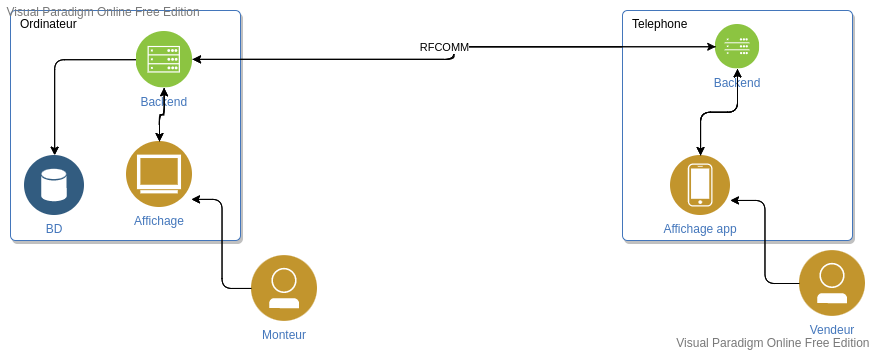
\includegraphics[scale=0.5]{images/architecture_ift592.png}

\subsection{Application mobile}
Tout projet Xamarin est divisé en trois projets.  Un projet pour le code partagé entre la version Android et iOS, un projet pour le code unique à Android et un projet pour le code unique à iOS.

Dans le cas des projets de code spécifique aux machines, la totalité du code est autogénérée par Xamarin, seules les images dans Ressources/drawable ont été ajoutées (les dossiers d’icônes sont propres au code machine). Tout le  travail a été effectué dans le code partagé.

Le code est séparé en 4 dossiers, Models, Services, ViewModels et Views. Models contient les classes d’objets, Services contient une banque de données temporaires, Views contient l’UI en xaml des pages des pages de l’application et ViewModels contient le code qui interagit avec ces pages.

L’application est composée de 4 pages. La page principale est la page commande. Sur cette page, toutes les commandes que l’ordinateur a sont affichées dans une liste. Cliquer sur un élément de la liste nous amène vers la page de nouvelle commande avec les champs déjà remplis. Il est donc possible de consulter les détails d’une commande et de la modifier si le client a changé d’idée en cliquant sur la commande dans la liste. Dans le coin en haut à droite, il y a un bouton plus qui nous amène vers la page de nouvelles commandes et nous permet ainsi de créer une nouvelle commande. Ainsi qu’un bouton « refresh » qui nous permet de mettre à jour la liste de commande. Toutes les pages de l’application ont également une ligne rouge apparaissant si l’application n’est pas connectée. Ainsi, l’utilisateur sait en tout temps s’il est connecté ou non. De même chaque page (sauf nouvelle commande) contient un menu dérouillant dans le coin gauche permettant de naviguer entre les pages.

Il y a également la page nouvelle commande, la page est composée de nombreux champ permettant de remplir les détails de la commande ainsi que de 4 boutons au bas de la page. Le bouton « livraison/sur place » change la commande entre à livrer ou à faire sur place. Si la commande est à livrer, des champs supplémentaires s’affichent, sinon ils sont cachés. Le bouton adressé précédent remplit les détails de livraison avec ceux de la précédente commande, ainsi si un client veut faire livrer plusieurs photos, il n’a pas à remplir les champs d’adresse plusieurs fois. Le bouton « cancel » annule la création de la commande et le bouton « save » envoie la commande à l’ordinateur. Le champ forfait et format sont des champs avec une liste de sélection. À l’origine la liste du champ format est vide, à la sélection d’un forfait, une liste de format disponible avec ce forfait sera disponible dans le champ format. Il en est de même pour les champs pays et province. Il est possible de choisir entre le Canada et les États-Unis et selon le choix, la liste des provinces/états sera différente.

Une autre page est la page paramètre. La est composé d’un seul bouton « scan ». Lorsqu’il est cliqué, une liste de tous les appareils avec lequel le mobile a déjà été lié via Bluetooth apparait. Pour qu’un appareil apparaisse dans la liste, il doit déjà avoir été « pair » avec le mobile une fois via l’application « paramètre » de l’appareil. Cliquer sur un élément de la liste nous connectera à l’appareil choisi via Bluetooth.

La dernière page est la page photo. Cette page et les fonctions y étant liées n’ont pas pu être complétées. La page devait pouvoir afficher une liste de dossier provenant de l’ordinateur. En cliquant sur un dossier, on devait pouvoir voir le contenu. Si ce qu’on cliquait est une photo, la photo aurait dû afficher. Le but de la page était de pouvoir consulter les photos de l’événement sur l’ordinateur. Cette fonctionnalité était une fonctionnalité supplémentaire que l’on voulait implémenter si on avait le temps, mais le temps à manquer.


\subsection{Tentative d'utilisation du BLE}
Dans un premier temps, nous nous sommes orientés vers le Bluetooth low energy car il semble correspondre plus à notre besoin principal. Le transfert de données très léger avec peu d'énergie. On a assez rapidement réussi à connecter les deux appareils, mais impossible de se connecter à un service défini par le protocole. Donc impossible de récupérer des données. La librairie de google implanté dans chrome (https://web.dev/bluetooth/).
On a également utilisé des applications de simulation de devise en BLE sur le téléphone pour tester, sans résultats. Encore à ce jour nous savons que ce n’est pas possible de communiquer avec ce protocole entre nos deux appareils, mais nous n'avons pas d'explication théorique pour le justifier. On suppose que la relation maitre/esclave ne s'établit pas bien entre deux appareils destinés à être dans la majorité des cas maitre. 

\subsection{Utilisation du bluetooth classique}
Après voir abandonner la piste du BLE. On s'est penché vers l'utilisation du Bluetooth classique. Pour nous amener vers cette piste on inspecter le code d'applications d'envois de message OpenSource en Bluetooth sur téléphone (Bluetooth Chat). On a remarqué que ce n'est pas le BLE qui est utilisé. À partir de ce moment, on a commencé à essayer des libraires pour ce type de Bluetooth sur l'application de bureau. Le premier problème rencontrer en nodejs est que toutes les librairies Bluetooth comme (node-Bluetooth, Bluetooth-serial-port) utilisent node-gyp. C'est un command-line tool qui permet de compiler des modules natifs en nodejs. Malgré de nombre heures de travail impossibles de réussir à faire compiler ces librairies pour les essayer et savoir si elles marchent. Node-gyp est connu pour avoir ce genre de problème, il faut la bonne version de nodejs, npm et python pour que tout marche correctement. Ainsi que la bonne version de la libraire. Beaucoup de dépendance qui augmente la possibilité de problème. Ne sachant même pas si ces librairies aller fonctionner on s'est tourné vers une autre approche du côté de l'ordinateur, c'est-à-dire faire fonctionner le Bluetooth en dehors du code avec uniquement des lignes de commandes simples. C'est à ce moment-là qu'on a découvert le protocole RFCOMM et réussi à faire notre première preuve de concept en ligne de command sur ligne et avec l'application de test sur Android : Serial Bluetooth.

Ouverture de la connexion sur Linux, puis connexion du téléphone.

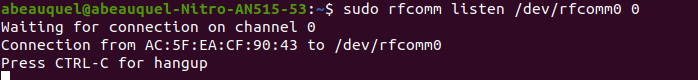
\includegraphics[scale=0.7]{images/rfcomm_connection_linux.png}


Envoi du message depuis le téléphone sur l'application Serial Bluetooth

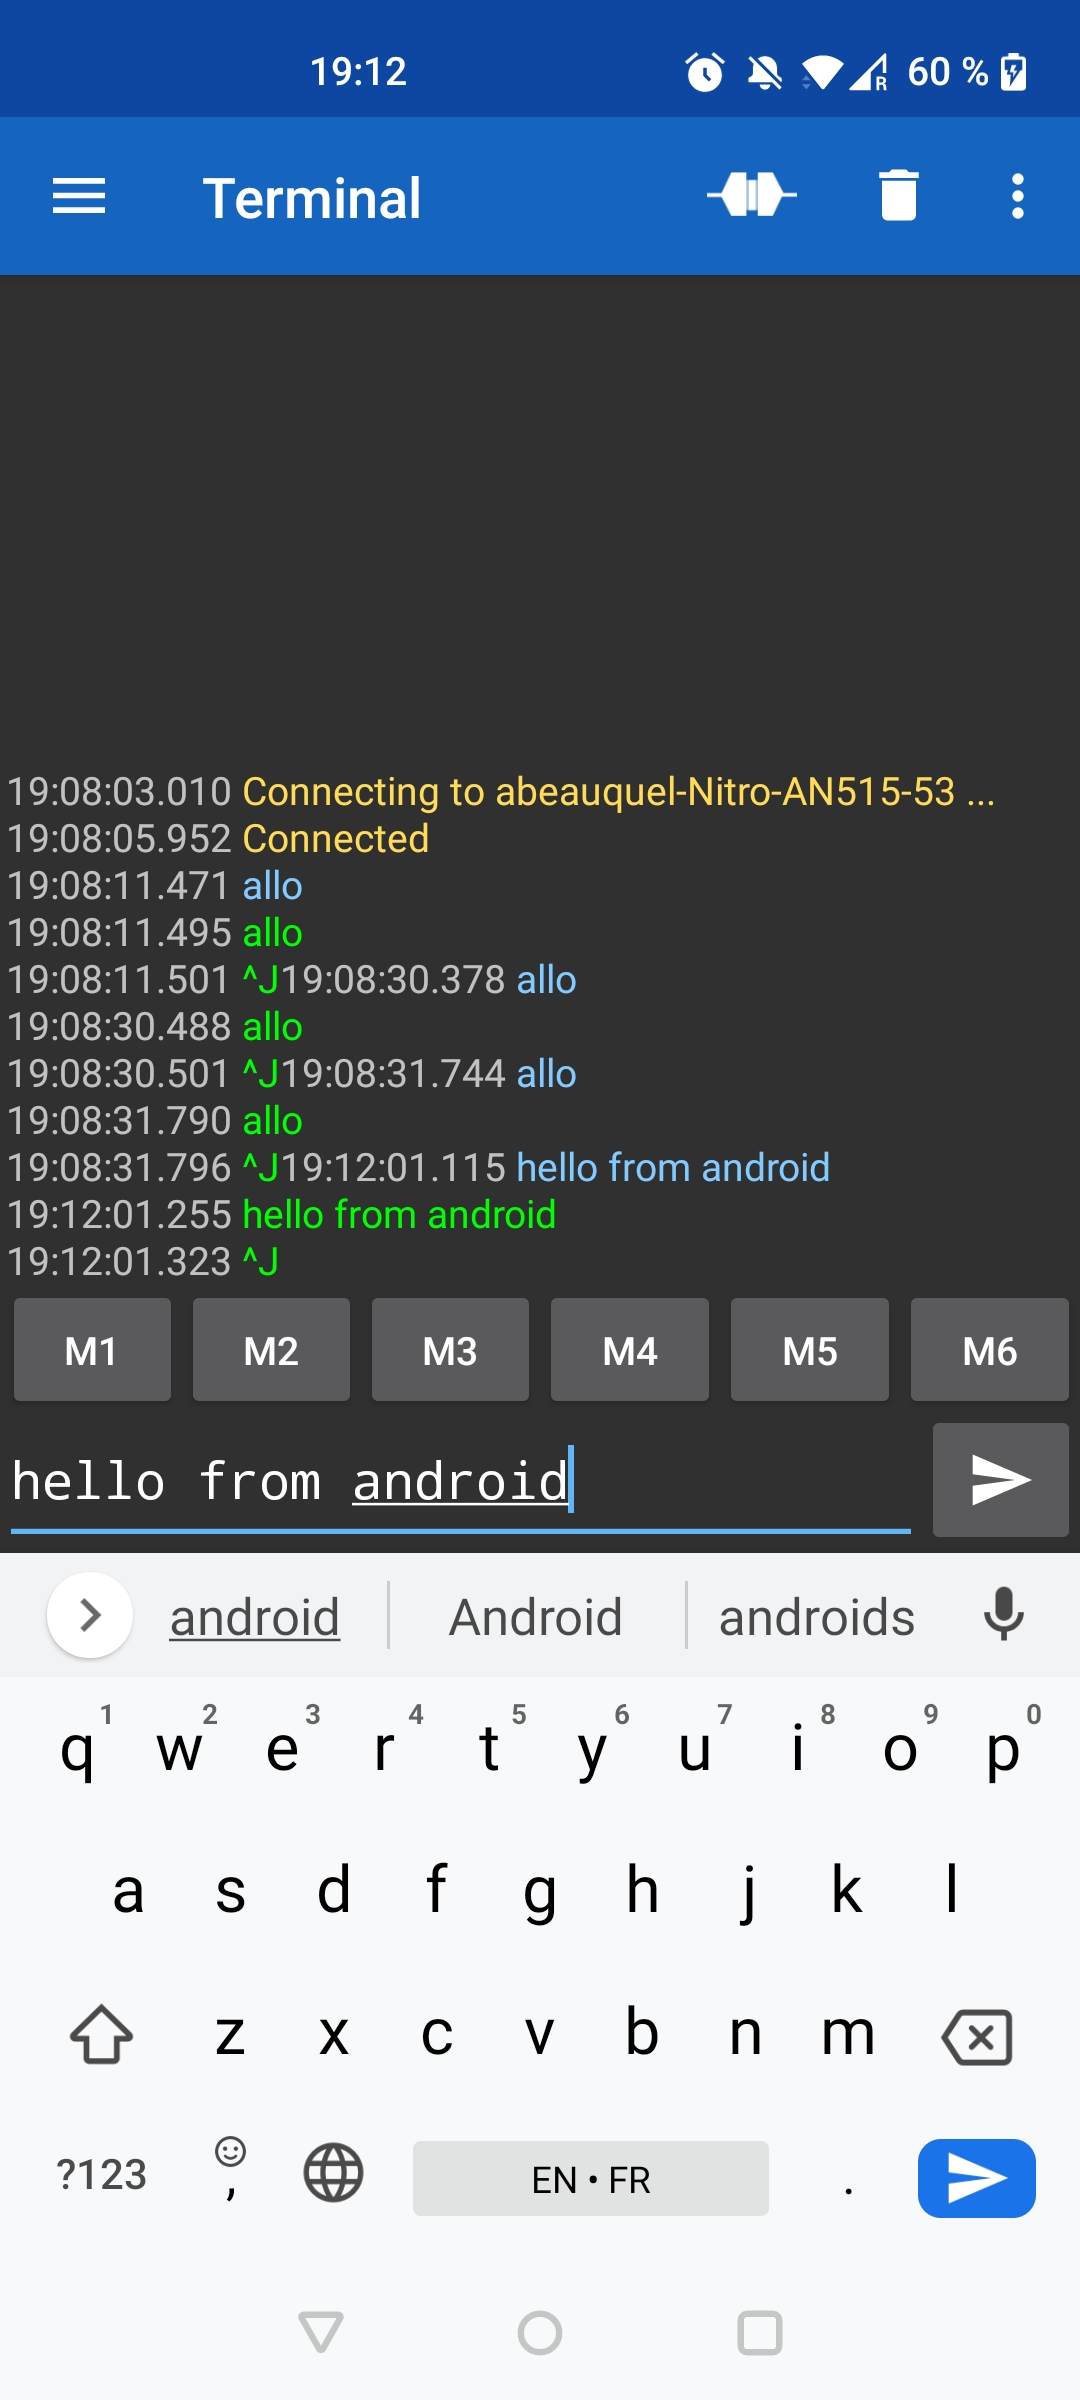
\includegraphics[scale=0.1]{images/rfcomm_telephone_message.jpg}

Lecture du message depuis linux

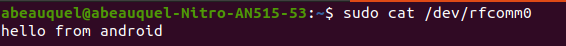
\includegraphics[scale=0.7]{images/rfcomm_linux_message.png}

Une fois cette preuve de concept réalisé, on a décidé d'implanter notre propre librairie avec ces appels systèmes. Pour l'application mobile, le fait de passer par Bluetooth classique plutôt que le BLE compliqua beaucoup la tâche. Les librairies natives pour le Bluetooth sont celles utilisées pour Windows qui ne fonctionnait pas.

Par contre Xamarin permet l'intégration de fichier .jar et d'interagir avec en C\#. Le Bluetooth a donc été développé en java. Pour le faire marcher, une class avec des méthodes static pour, voire les appareils disponibles, se connecter, envoyer des données et revoir des données a été créer. Cette classe s'occupa aussi d'instancier un nouvelle file d'exécution qui se relie à un socket pour l'envoi et la réception de donnée. 

Tout le code java est compilé avec la version 8 pour obtenir un .jar qu'il faut part la suite importer dans le projet pour que Xamarin puisse interagir avec. La synchronisation pour la réception de donnée posa un problème. Une difficulté supplémentaire pour la synchronisation est qu’étant donné que la librairie est précompilée dans le projet, elle devient une boite noire, il n'y a pas de fonction de débogage ni d'impression à l'écran. Les seules intégrations sont les méthodes de statice qui peuvent retourner d’abjects primitifs pour qu'ils puissent être facilement interprétés dans le code de l'application.

Au début, de l'attente active était utilisée pour passer le temps entre l'envoi du message à l'application de bureau et la réception de la réponse. 

Par la suite, les messages POSIX ont été regardés pour la communication interprocessus puisqu’Android possède un Kernel de Linux comme base. Les messages POSIX ne sont pas supportés puisqu'ils sont trop lourds et qu'Android possède sa propre librairie de c ce qui pose des problèmes. 

Par contre, java support les futures et les possède des exécuteurs qui peuvent attendre puis être notifier. L'idée pour enlever l'attente active était que lorsqu'un message est envoyé, un objet futur va nous donner la réponse lorsqu'elle arrivera. Puisqu'un fil écoute sur un socket, lorsqu'un message arrive, un événement est lancé avec le nouveau message qui notifie l'exécuteur de l'objecté futur pour qu'il puisse donner le résultat. Avec des tests manuels en mode débogage, cette version fonctionnait. Parfois un message devait être envoyé deux fois pour obtenir une réponse, mais le tout fonctionnait sans attente active. 

Par contre, lors de tests avec l'application de bureau, cette méthode était encore moins stable. Puisque la communication utilise un port série, avec des points d'arrêt et l'avancement manuel du code, le buffer du port série garde l'information donc le message arrive au complet. 

Cependant, lors de l'exécution, l'arrivée de chaque caractère peut lancer l'événement de l'arrivée d'un message. Il fallait donc trouver un moyen de s'assurer que le message était complet avant de renvoyer la réponse à l'application. Les massages sont envoyés en json, donc il est facile à le désiraliser et s'assurer que les champs sont valides. Une fonction a été crée pour que lorsqu'un nouveau message arrive, si le json est valide et possède les bon champs, l'exécuteur se fait notifier pour renvoyer le message. 

Ce design n'a jamais été suffisamment stable pour qu'il puisse être utilisé dans le projet. Puisque toute la logique et complexité se retrouve dans la librairie, les outils disponibles pour trouver les erreurs sont très limités, la librairie ne pouvait même pas écrire dans un fichier puisqu'il manquait le contexte d'Android requis pour l'écriture. Il fallut donc déplacer la logique dans l'application et laisser la librairie au minimum.

Finalement, pour la communication par Bluetooth dans l'application mobile, un service a été crée qui s'occupe d'envoyer le message, attendre X millisecondes, lire la réponse puis si le message n'est pas valide, il recommence le processus jusqu'a l’obtention d'un message valide. 

Le service fait une forme d'attente active ce qui cause l'application de ne pas répondre durant la communication par contre, cette version est stable et permet l'envoie et la réception de message.
\subsection{Fonctionnement du bluetooth dans le projet}
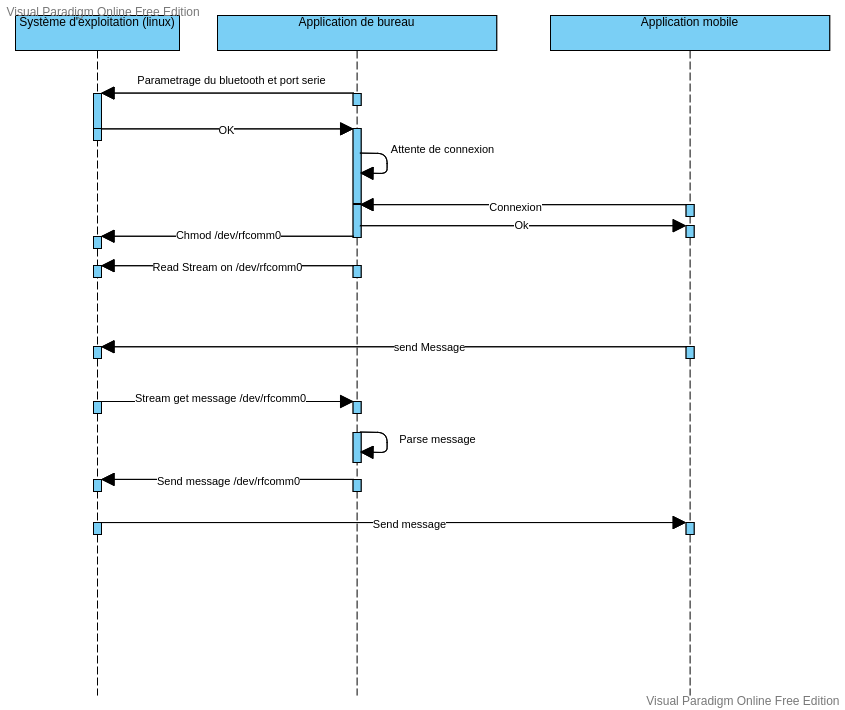
\includegraphics[scale=0.5]{images/sequence_bluetooth.png}

La fonction parseMessage sur l'application de bureau gère les messages suivant:
\begin{itemize}
\item Création d'une commande
\item Modification d'une commande
\item Demande de la liste des commandes
\item Demande d'un LS du dossier courant
\item Demande d'un CD dans sous dossier
\item Demande retour au dossier parent
\item Demande recuperation d'une image
\end{itemize}
L'application peut donc renvoyer au mobile les messages suivant :
\begin{itemize}
\item Liste des commandes
\item LS du dossier courant
\item CD dans sous dossier
\item Retour au dossier parent
\item Image
\end{itemize}

\subsection{Resultat obtenue}
Au final les 2 applications (mobile et ordinateur) sont finies. Les objectifs de base sur ce que l’application peut faire sont accomplis. La communication entre les applications sont fonctionnelle et la fonction de prendre des commandes sur mobile et les consulter sur l’ordinateur marche.

Toutefois, un grand nombre de problèmes a été rencontré. L’objectif d’avoir nos applications sur iOS et OSX n’ont pas été rempli. L’application mobile et le protocole Bluetooth associé ne sont fonctionnels que sur Android. De même, l’application bureau et son protocole Bluetooth ne sont fonctionnelle que sur Linux. L’objectif bonus de pouvoir consulter les photos de l’ordinateur sur le mobile n’est pas complété.


\subsection{Analyse des resultats}
L’objectif initial du projet était d’avoir l’application mobile sur iOS. L’application était d’abord développée sur Android, puisque le développement sur Android est plus facile (impossible de tester iOS sur Windows), puis porté sur iOS. L’utilisation de la framwork rendant le port vers iOS facile.

Le port de l’application vers iOS ne cause aucun problème en lui-même. Or, lorsque nous avons commencé à porter l’application, nous avons rencontré un problème qui a mis en doute l’utilité de porter l’application sur mobile. Le problème est que pour déployer une application sur un appareil iOS, il faut absolument avoir un compte Apple avec le developper program. Ce programme coûte 100 USD/années. Puisque l’application ne requiert pas vraiment de puissance, l’achat d’une tablette Android basique serait plus économique pour le client dès la première année d’utilisation. Ce problème a été rencontré très tard, car pour pouvoir tester l’application sur un émulateur iOS, il faut être sur mac et c’est lorsque nous avons testé sur mac que nous avons rencontré le problème. Nos recherches au début du projet nous avaient laissés croire que nous n’aurions pas ce problème, mais ça s’est avéré faux.

Pour le Bluetooth de l'application mobile étant donné qu'il est fait dans une librairie en java pour Android, il n'est pas supporter sur IOS. Il aurait fallu recoder la librairie en Swift et faire un processus similaire pour l'intégrer dans l'application Xamarin. Il aurait aussi fallu changer de protocole puisque rfcomm est obsolète sur IOS et OSX pour des raisons de sécurité. Changer de protocole ne sera pas compliquer puisque la communication entre les produits Apple se fait facilement. Par contre ses difficultés s'ajoutent au problème économique du déploiement sur IOS.

Au final, avec l’accord du client, le choix a été fais que l’application resterait seulement sur Android et qu’il s’achèterais une tablette Android.

%abandon du crossplateforme




\section{Conclusion}
Pour conclure, nous avons sous-estimé l’effort requis pour faire une communication Bluetooth, particulièrement dans le cas du cross-plateforme. Nous avions choisi d’utiliser le Bluetooth, car il respectait les contraintes, mais aussi par défi. Le Bluetooth était une nouvelle technologie que nous n’avions jamais utilisée et a été la partie la plus compliquée de l’application et le défi a été plus grand qu’on pensait. De même, le développement sur macOS et iOS a été sous-estimé. Jamais nous n’aurions pensé que c’était si compliqué de programmer pour des appareils Apple (Apple Developper Program requis, iOS doit être testé sur mac, un protocole Bluetooth aurait dû être en Switft et donc n’aurait pu être programmé que sur un mac, etc.). Beaucoup de choses n’ont pas été prises en compte au début du projet et ça nous a coûté beaucoup de temps.

Au final, on a une application de base fonctionnelle, mais qui ne peut être utilisé par le client puisqu’elle ne fonctionnera pas sur ces machines. Compléter l’application requérait de refaire tous les protocoles Bluetooth pour iOS et macOS se qui est impossible vu le manque d’accès à une machine utilisant macOS. Or, lors de la présentation finale, quelqu’un nous a donné une solution qui réglerait nos problèmes tous en respectant les contraintes initiales. Il serait possible d’utiliser l’ordinateur pour générer un réseau local privé auquel l’appareil mobile pourrait se connecter. Les ressources pour la communication par internet étant beaucoup plus standardisé, il serait beaucoup plus facile de finir l’application en utilisant cette méthode. C’est une méthode dont nous ignorions l’existence jusqu’à maintenant, mais qui aurait énormément simplifié le développement.

Au final, le livrable pour le client n’est pas fonctionnel, mais puisque ce projet est surtout un projet personnel d’un des membres de l’équipe pour un membre de son entourage (il voulait faire une application pour l’aider), le projet sera complété en dehors du cadre de l’université. Nous nous sommes lancé dans un projet utilisant des technologies que nous ne connaissions pas, beaucoup de problèmes ont été rencontrés, mais de même beaucoup a été appris, que ce soit au niveau du Bluetooth ou du cross-plateforme.

\section{Annexes}

\begin{figure}[H]
  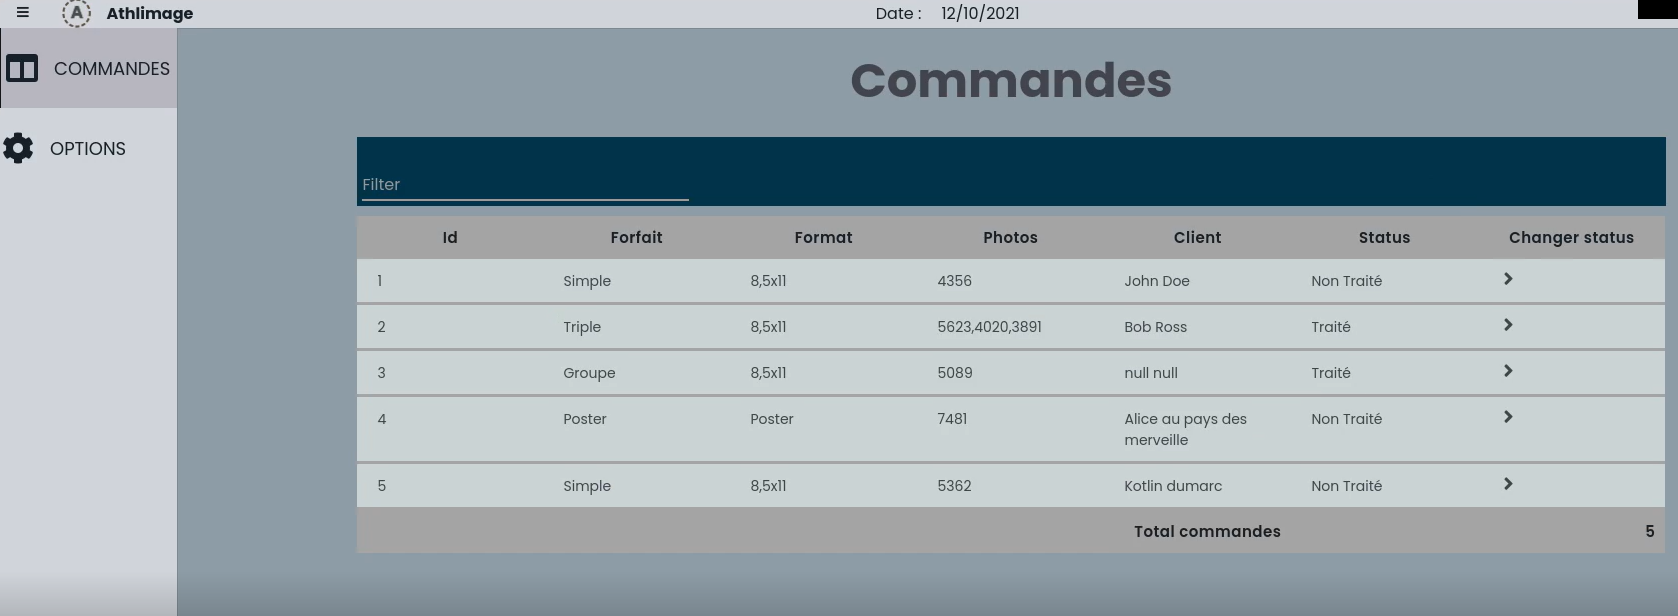
\includegraphics[width=\textwidth]{images/AppBureau.png}
  \caption{L'application bureau}
\end{figure}

\begin{figure}[H]
  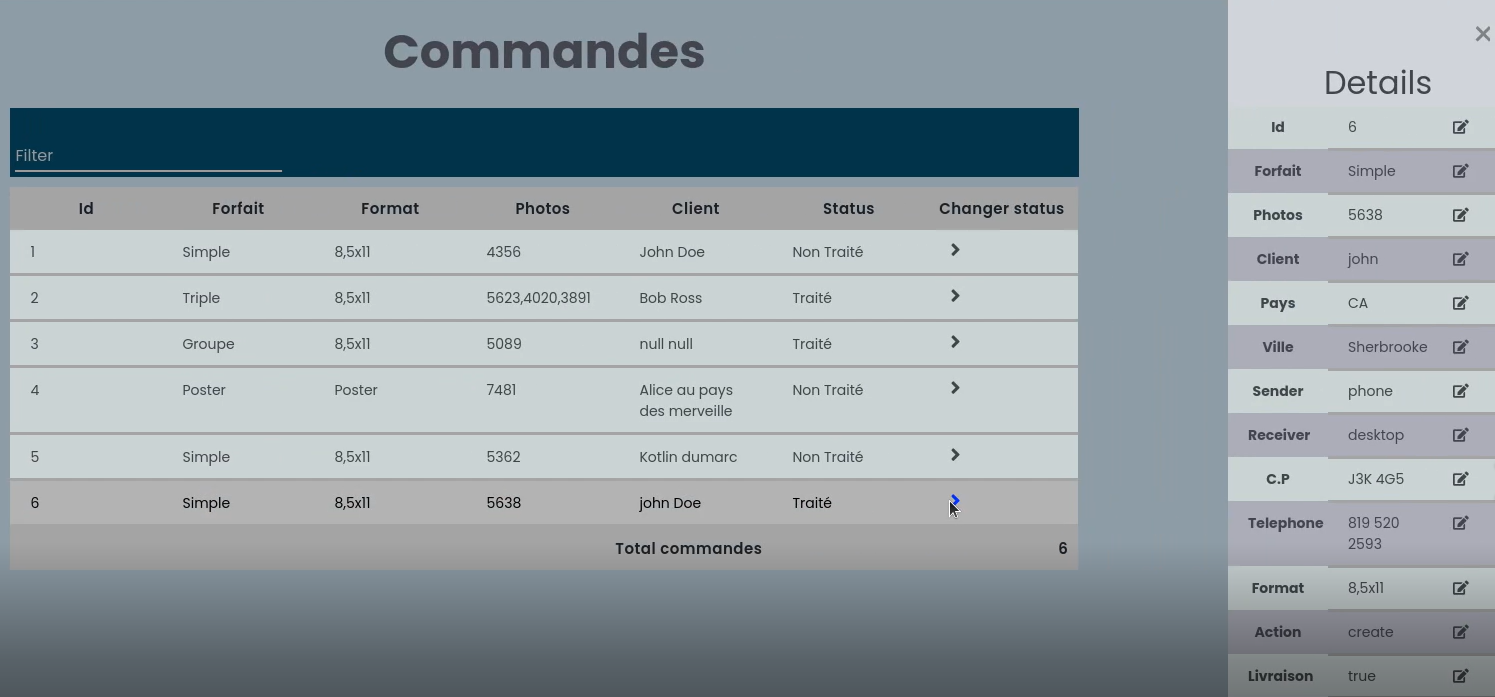
\includegraphics[width=\textwidth]{images/AppBureauDetail.png}
  \caption{L'application bureau, vue détaillée d'une commande}
\end{figure}

\begin{figure}[H]
  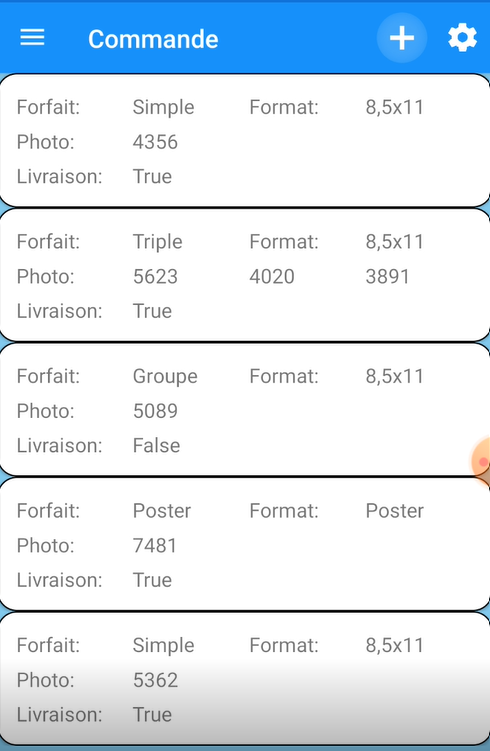
\includegraphics{images/AppMobileMainScreen.png}
  \caption{L'application Mobile,` l'écran principale}
\end{figure}

\begin{figure}[H]
  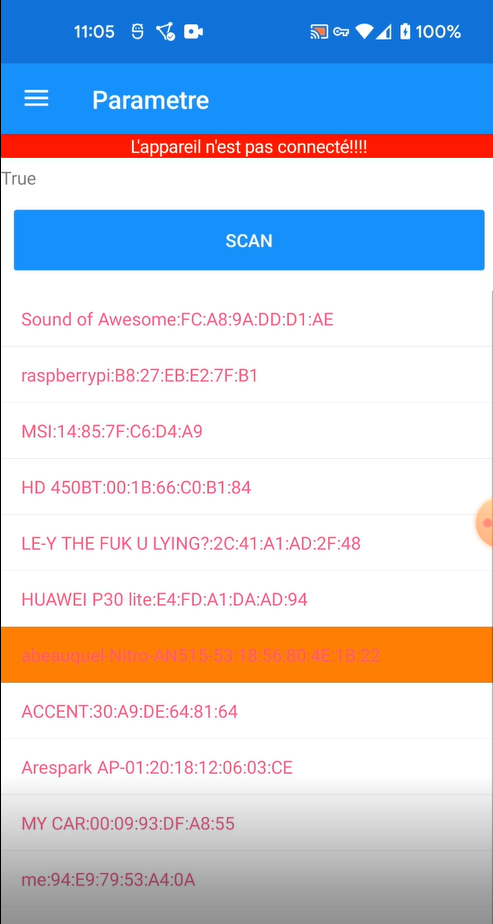
\includegraphics{images/AppMobileSetting.png}
  \caption{L'application mobile, page de connection}
\end{figure}

\begin{figure}[H]
  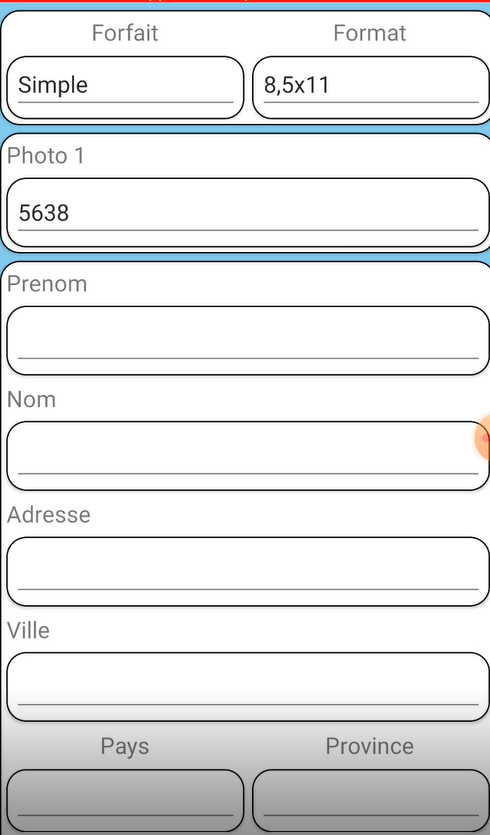
\includegraphics{images/AppMobileNewCommand.png}
  \caption{L'application mobile, prise d'une nouvelle commande}
\end{figure}
\newpage

\section{Bibliographie}
\vspace{-0.75cm}
\renewcommand\refname{}

\bibliographystyle{plain-fr}
\bibliography{bibliographie}
\nocite{*}


\end{document}
